%%%%%%%%%%%%%%%%%%%%%%%%%%%%%%%%%%%%%%%%%%%%%%%%%%%%%%%%%%%%%%%%%%%%%%%%%%%%%%%%
%2345678901234567890123456789012345678901234567890123456789012345678901234567890
%        1         2         3         4         5         6         7         8
\documentclass[letterpaper, 10 pt, conference]{ieeeconf}  % Comment this line out
                                                          % if you need a4paper
%\documentclass[a4paper, 10pt, conference]{ieeeconf}      % Use this line for a4

\usepackage{float}
                                                          % paper
% uso paquete bookmark para tener bien los outlines.
\usepackage{bookmark}

% Configuro el idioma.
\usepackage[utf8]{inputenc} % Importante para mantener acentos.
\usepackage[spanish, activeacute]{babel} % Requiere: texlive-lang-spanish. Por primera vez hay que ejecutar: texconfig init> log

% Paquete para poder usar acentos en $$.
\usepackage{mathtools}
%\setmathfont{XITS math}

% Para los diagramas de flujo
\usepackage{tikz}
\usetikzlibrary{shapes.geometric, arrows}

% Elementos del diagrama
\tikzstyle{startstop} = [rectangle, rounded corners, 
minimum width=6em, 
minimum height=2em,
text centered, 
draw=black, 
fill=red!30]

\tikzstyle{io} = [trapezium, 
trapezium stretches=true, % A later addition
trapezium left angle=70, 
trapezium right angle=110, 
minimum width=6em, 
minimum height=2em, text centered, 
draw=black, fill=blue!30]

\tikzstyle{block} = [rectangle, 
minimum width=8em, 
minimum height=3em, 
text centered, 
text width=7.5em, 
draw=black, 
fill=white!30]

\tikzstyle{def} = [rectangle, 
minimum width=14em, 
minimum height=3em, 
text centered, 
text width=12em, 
draw=black, 
fill=purple!30]

\tikzstyle{swap_proccess} = [rectangle, 
minimum width=8em, 
minimum height=2em, 
text centered, 
text width=8em, 
draw=black, 
fill=orange!30]

\tikzstyle{process} = [rectangle, 
minimum width=6em, 
minimum height=2em, 
text centered, 
text width=6em, 
draw=black, 
fill=orange!30]

\tikzstyle{decision} = [diamond, 
minimum width=6em, 
minimum height=6em, 
text centered, 
draw=black, 
fill=green!30]
\tikzstyle{arrow} = [thick,->,>=stealth]

\usepackage{siunitx}

% package to get \url
\usepackage{hyperref}
\hypersetup{
  colorlinks=true,
  linkcolor=magenta,
  filecolor=magenta,
  citecolor=magenta,      
  urlcolor=magenta,
}

% Graficos electrónicos
\usepackage[RPvoltages]{circuitikz}

\IEEEoverridecommandlockouts                              % This command is only
                                                          % needed if you want to
                                                          % use the \thanks command
\overrideIEEEmargins
% See the \addtolength command later in the file to balance the column lengths
% on the last page of the document

\usepackage{graphicx}
\usepackage{graphics}

% styling for matlab/octave code.
\usepackage{matlab-prettifier}
% Configuracion, con esto puede agregar ñ.
\lstset{
  literate={ñ}{{\~n}}1
}

\usepackage{listings}

% The following packages can be found on http:\\www.ctan.org
%\usepackage{graphics} % for pdf, bitmapped graphics files
%\usepackage{epsfig} % for postscript graphics files
%\usepackage{mathptmx} % assumes new font selection scheme installed
%\usepackage{times} % assumes new font selection scheme installed
\usepackage{amsmath} % assumes amsmath package installed
%\usepackage{amssymb}  % assumes amsmath package installed

\title{\LARGE \bf Trabajo de Aplicación}

\author{
  Tom\'as Vidal, Lautaro Frangi, Thomas Sille\\
  {\small Grupo 10}\\
  {\it Control Automático III}\\
  {\it Facultad de Ingenier\'ia, UNLP, La Plata, Argentina.}\\
  {\it 25 de Noviembre, 2024.}
}                                            % <-this % stops a space

\begin{document}
\maketitle
\thispagestyle{empty}
\pagestyle{empty}

\section{Introducción}
El siguiente informe describe la realización del trabajo de aplicación asignado a los alumnos de control automatico III, el mismo está dividido en dos secciones la primera que tiene que ver con la identificación de sistemas para una planta dada y una segunda en donde se realizara un paso a paso de la construcción de un un controlador PID para la misma.

\section{Identificación de sistema}

\subsection{Simulación del sistema}
En esta instancia, se simuló la planta con el objetivo de poder efectuar un análisis de su comportamiento. Esto se realizó en el programa de diseño de circuitos electrónicos y digitales Proteus Design Suite, el mismo nos permitió diseñar y corroborar el correcto funcionamiento de los algoritmos implementados para la síntesis de las diferentes señales de entrada a la planta. Debido a que la planta cuenta con seis componentes capaces de almacenar energía (capacitores), la misma puede modelarse como un sistema lineal de sexto orden. Cada etapa está separada por un amplificador operacional realimentado negativamente y alimentado con cinco voltios. 

\begin{figure}[htpb]
  \centering
  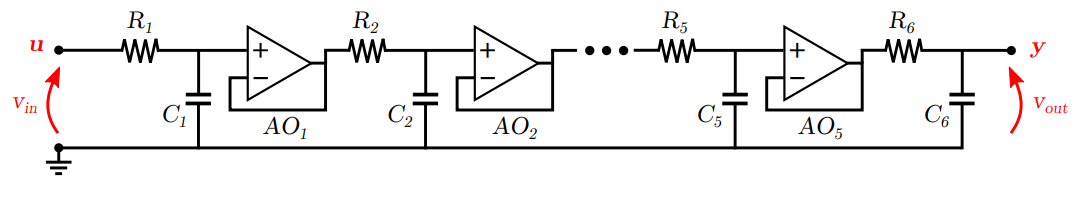
\includegraphics[width=0.43\textwidth]{./IMAGENES/diag_placa.png}
  \caption{Esquemático de la placa}
  \label{fig:placa}
\end{figure}

\subsection{Respuesta al escalón}
Se empleó una señal PWM con ciclo de trabajo del $20\%$, para hacer que la entrada vaya de 0V a 1V (en el segundo 0), luego de que se estableciera la salida (a los 3 segundos), se cambió el PWM al $80\%$ de manera que actuará como escalón, y luego de pasados 3 segundos, se volvió a llevar el ciclo de trabajo al $20\%$. Esto se realizó tanto en simulación (en Proteus), como en la placa física, como los datos son idénticos para ambos casos, de ahora en adelante se referirá solamente a los datos.

\begin{figure}[htpb]
  \centering
  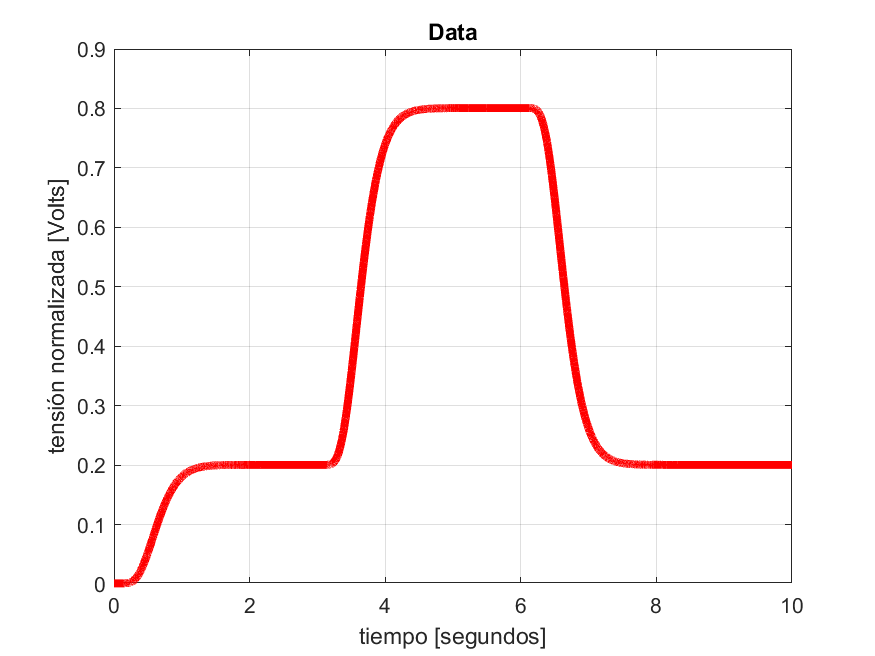
\includegraphics[width=0.43\textwidth]{./imagenes/datos_resp_escalon.png}
  \caption{Respuesta al escalón del sistema (\textit{normalizada a 5V})}
  \label{fig:resp_esc}
\end{figure}

\subsection{Modelos de la planta}
Una vez hecho el relevamiento de los datos, se emplearon para obtener un modelo de la planta original de alto orden, uno del tipo FOPDT\footnote{First order plus dead time: primer orden más tiempo muerto} y otro SOPDT\footnote{Second order plus dead time: segundo orden más tiempo muerto}, para esto utilizamos la aplicación de Matlab System Identification\footnote{Herramiento de MATLAB Toolbox que permite hacer identificación de sistemas} habiendo previamente procesados los datos (se tuvo que linealizar el tiempo).

\subsubsection{Modelo FOPDT}
\begin{equation}
  \frac{e^{-0.33791s}}{0.28802s+1}
\end{equation}

\subsubsection{Modelo SOPDT}
\begin{equation}
  \frac{e^{-0.24087}}{(0.18561+1)(0.18561+1)}
\end{equation}

\subsubsection{Modelo de orden 6}
\begin{equation}
  \tiny{\frac{1.261*10^6}{s^6+75.11s^5+1869s^4+2.523104s^3+1.888105s^2+7.568105s^+1.26106}}
\end{equation}

\vspace{1em}

\subsubsection{Precisión de los modelos}


\begin{table}[htpb]
\centering
\begin{tabular}{|l|c|c|c|}
\hline
\textbf{Tipo} & \multicolumn{1}{l|}{\textbf{EFP}}     & \multicolumn{1}{l|}{\textbf{EMC}}     & \multicolumn{1}{l|}{\textbf{fit porcentual}} \\ \hline
FOPDT   & 0.001008                     & 0.01007                      & 91.97\%                             \\ \hline
SOPDT   & 0.0002428                    & 0.0002421                    & 96.06\%                             \\ \hline
Orden 6 & $3.963*10^{-9}$ & $3.912*10^{-9}$ & $99.98\%$                             \\ \hline
\end{tabular}
  \caption{Precisión de los modelos}
  \label{tab:precision_modelos}
\end{table}

Es importante tener en cuenta que estos modelos están \textbf{normalizados} con respecto a 5V. \\

\textit{Para corroborar la precisión de los modelos, se obtuvieron más datos con otro escalón, con los que se hicieron las verificaciones y cálculos.}
Los resultados de estos modelos se presentan en la figura \ref{fig:resp_esc_modelos}, para hacer una mejor interpretación de los datos y los modelos, se centró la respuesta al escalón de los datos entre 1V y 4V, y entre 3 y 6 segundos.

\begin{figure}[htpb]
  \centering
  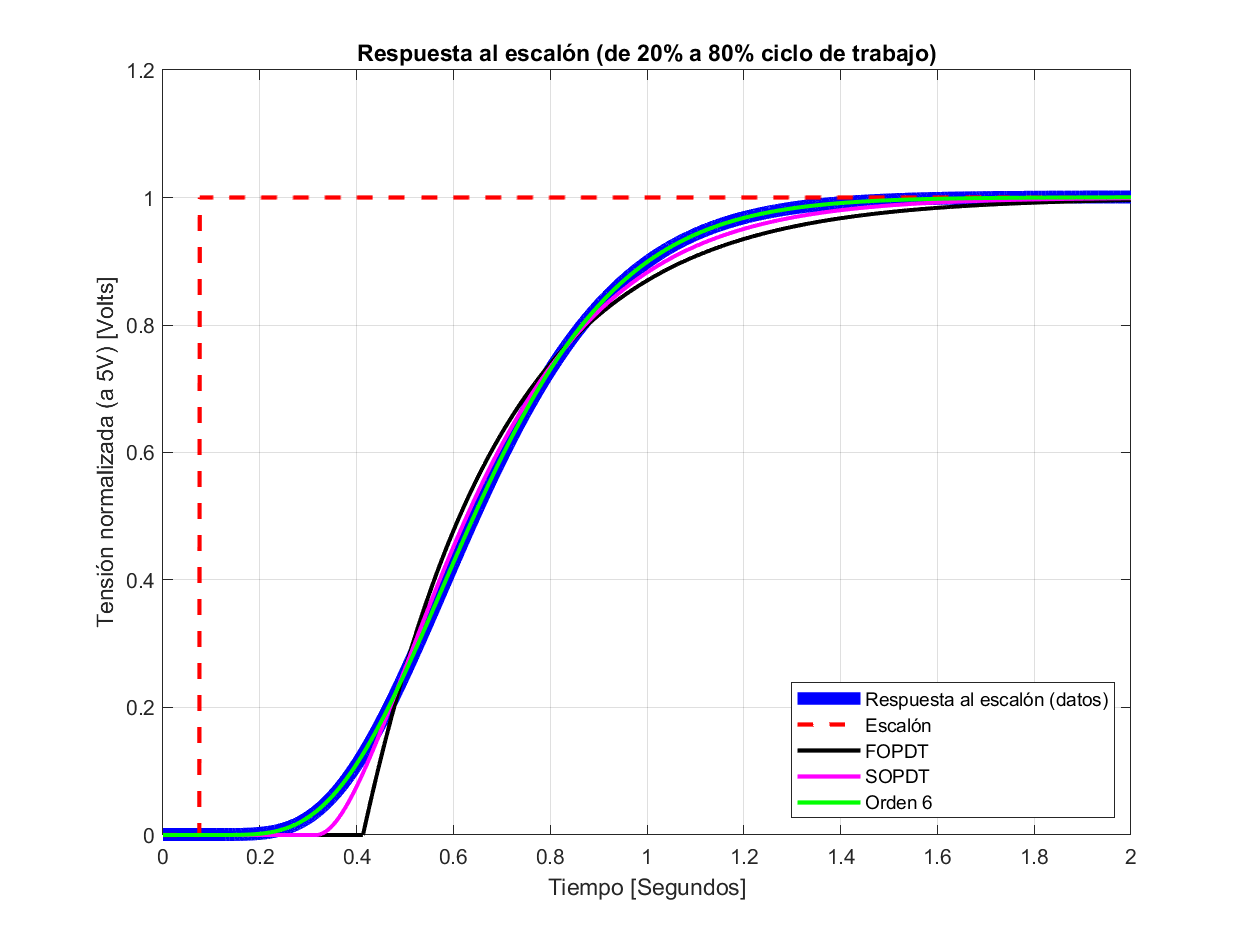
\includegraphics[width=0.43\textwidth]{./IMAGENES/resp_esc.png}
  \caption{Respuesta al escalón de los modelos}
  \label{fig:resp_esc_modelos}
\end{figure}

\subsubsection{Análisis de robustez}

Considerando una tolerancia de los elementos del circuito de un $10\%$ (al ser el producto de estos, termina siendo la suma, es decir una tolerancia del $20\%$) y partiendo del modelo de orden 6, es posible establecer una familia de modelos a partir de un peso de incertidumbre dinámica global. Se consideró un peso de \textbf{incertidumbre aditiva}, ya que el mismo es el más adecuado a la hora de aproximar un modelo de orden elevado con otro de orden reducido. La condición a evaluar para el diseño del peso es la siguiente:

\begin{equation*}
  |G(jw) - G_0(jw)| < |W\delta(jw)|
\end{equation*}

Donde G es la familia de plantas y $G_0$ se obtiene a partir del modelo FOPDT obtenido. Entonces graficando esta condición para distintos valores para la constante de tiempo de G
se obtuvo la siguiente función peso:

\end{document}